\section{Introduzione}
\fancyhead[RO,LE]{Introduzione}

La crescita del traffico stradale e la capacità limitata delle infrastrutture autostradali rappresentano sfide sempre più pressanti per le società moderne. L'incremento costante del numero di veicoli in circolazione ha portato a una saturazione sempre maggiore delle strade, ma anche a un aumento della durata degli spostamenti, con conseguenti ritardi, stress per gli automobilisti e impatti negativi sull'ambiente dovuti alle emissioni generate dal traffico fermo. In questo contesto, la ricerca di soluzioni innovative e efficienti per migliorare la gestione del traffico stradale è diventata sempre più importante.
\newline
Tra le molteplici strategie proposte per affrontare questo problema, una delle più promettenti è il concetto di platooning di veicoli. Detto anche convogliamento, consiste nell'allineamento e nella gestione coordinata di più veicoli in movimento lungo una strada. Questa formazione di veicoli segue un veicolo guida, cercando di mantenere una distanza costante prestabilita e ridotta tra di loro e minore in confronto alla distanza di si, e risponde in modo coordinato alle variazioni di velocità e direzione del veicolo di testa. Questo approccio offre numerosi vantaggi, tra cui una maggiore efficienza nel flusso del traffico, una riduzione della distanza tra i veicoli stessi e un miglioramento della sicurezza stradale.
\newline
Tuttavia, la piena realizzazione del potenziale del platooning richiede l'adozione di sistemi avanzati di controllo e automazione dei veicoli. In particolare, è fondamentale sviluppare algoritmi e tecnologie in grado di coordinare in modo efficace e sicuro il movimento dei veicoli all'interno del convoglio, garantendo contemporaneamente il rispetto delle normative stradali e la massima sicurezza per i conducenti e gli altri utenti della strada.
\newline
A questo scopo, il controllo di crociera adattivo e cooperativo (CACC) si presenta come una soluzione promettente. Questo sistema utilizza dati provenienti dai veicoli stessi, oltre a informazioni ottenute da sensori come telecamere, radar e lidar (scanner laser), per regolare automaticamente la velocità e la distanza tra i veicoli all'interno del convoglio. Grazie alla sua capacità di scambio di dati wireless tra veicoli, il CACC consente di mantenere intervalli di tempo significativamente inferiori rispetto ai sistemi di controllo di crociera adattivi tradizionali, contribuendo così a aumentare la capacità delle strade e a ridurre il consumo di carburante.
\newline
Da annoverare fra i vantaggi bisogna vagliare il caso in cui ci sia bisogno di frenare bruscamente, se c'è una persona alla guida c'è da tenere conto del tempo di reazione, calcolato mediamente in un range fra $1s$ e $1.1s$ che corrisponde però a una distanza maggiore proporzionalmente alla velocità a cui si sta viaggiando, come mostrato in figura:
\begin{figure}[H]
    \centering
    \captionsetup{justification=centering, margin=2cm}
    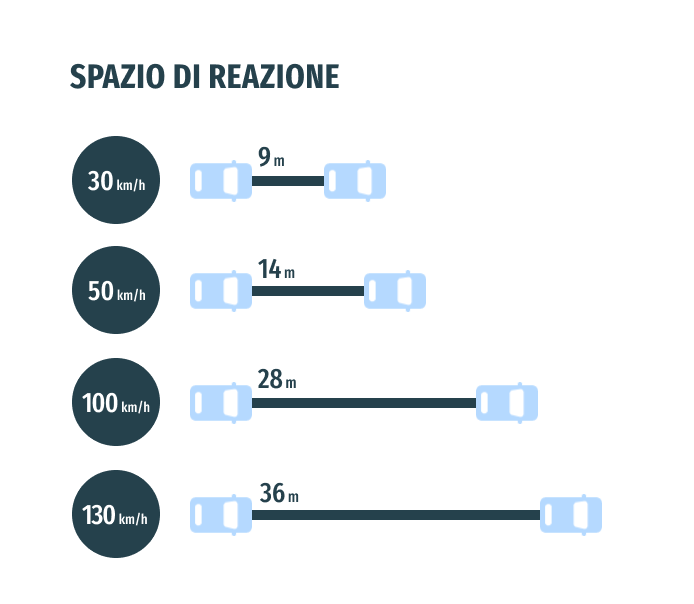
\includegraphics[width=0.75\textwidth]{images/1-introduction/spazio-reazione.png}
    \caption{Spazio di reazione di un veicolo con guidatore umano con tempo di reazione $1s$ \cite{distanza_sicurezza_autoscuola_quattroruote}}
    \label{fig:spazio-reazione}
\end{figure}
\noindent quindi considerando anche lo spazio di frenatura come mostrato in figura

\begin{figure}[H]
    \centering
    \captionsetup{justification=centering, margin=2cm}
    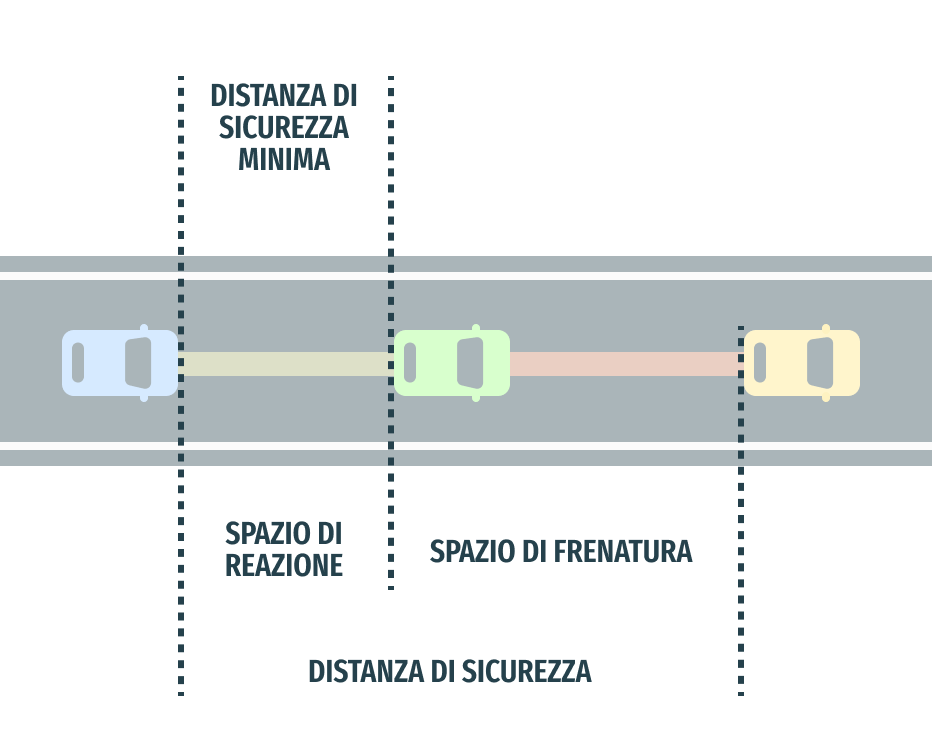
\includegraphics[width=0.8\textwidth]{images/1-introduction/distanze-sicurezza-spazi.png}
    \caption{Componenti distanza di sicurezza \cite{distanza_sicurezza_patentino_online}}
    \label{fig:distanze-sicurezza-spazi}
\end{figure}

\noindent Tuttavia, nonostante i suoi evidenti vantaggi, l'implementazione efficace del CACC e dei sistemi di platooning richiede la progettazione e lo sviluppo di un frontend sofisticato e efficiente per la simulazione e la valutazione delle prestazioni di tali sistemi. È qui che il nostro progetto entra in gioco. Ci proponiamo di sviluppare un frontend innovativo per la simulazione del platooning di veicoli, concentrandoci sull'ottimizzazione del modello fisico e del sistema di controllo, al fine di massimizzare l'efficienza del traffico stradale, garantendo al contempo la massima sicurezza per tutti gli utenti della strada.

\begin{figure}[H]
    \centering
    \captionsetup{justification=centering, margin=2cm}
    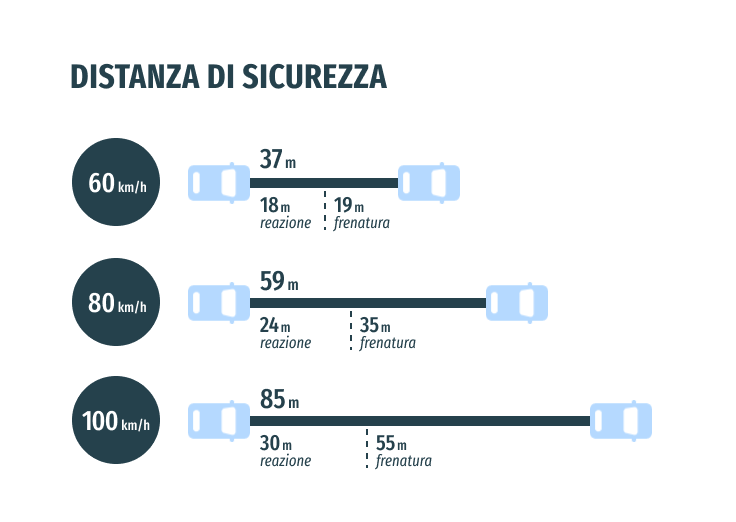
\includegraphics[width=0.8\textwidth]{images/1-introduction/distanza-sicurezza.png}
    \caption{Distanza di sicurezza \cite{distanza_sicurezza_autoscuola_quattroruote}}
    \label{fig:distanza-sicurezza}
\end{figure}
